\newpage
\null
\thispagestyle{empty}
\newpage

\addcontentsline{toc}{chapter}{1 Peter}

% Safely inserts your illustration full-bleed on its own page.
% This completely bypasses the page builder, headers, and geometry bugs!
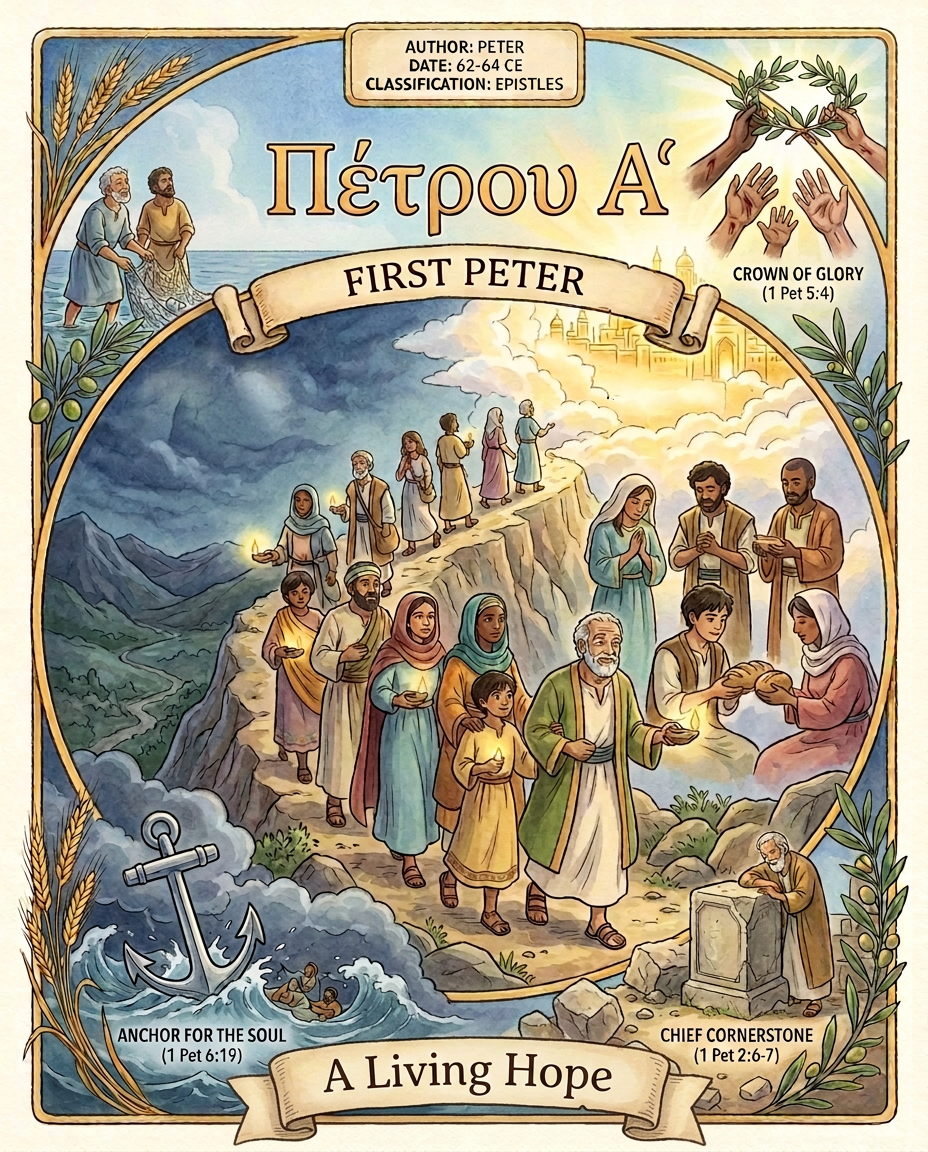
\includepdf[pages=1, fitpaper=false, width=\paperwidth, height=\paperheight, , keepaspectratio=false]{images/divider2/1peter2.png}
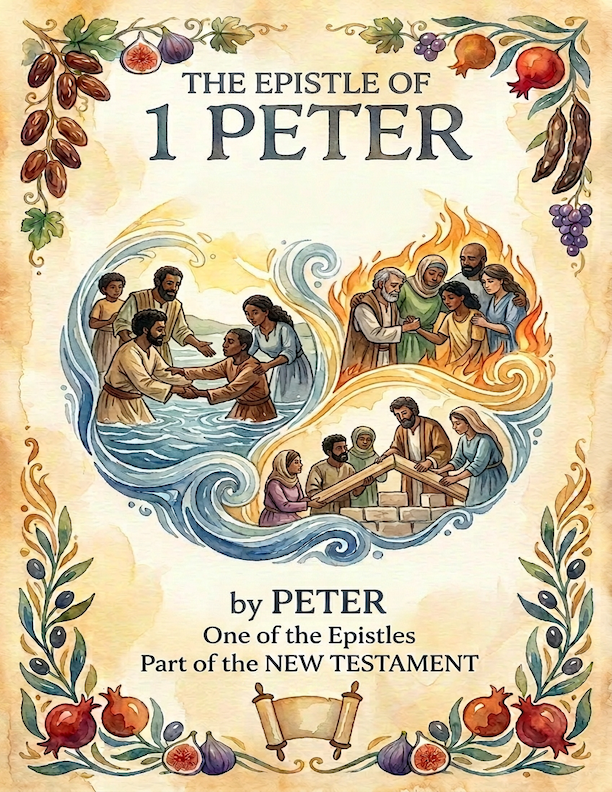
\includepdf[pages=1, fitpaper=false, width=\paperwidth, height=\paperheight, , keepaspectratio=false]{images/divider1/1peter.png}

\includepdf[pages=1, fitpaper=false, width=\paperwidth, height=\paperheight, , keepaspectratio=false]{images/8.5x11-Dot-Grid.png}

\includepdf[pages=1, fitpaper=false, width=\paperwidth, height=\paperheight, , keepaspectratio=false]{images/8.5x11-Dot-Grid.png}
\mybook{1 Peter}
\vspace{-1.36in}


\mychapter{} \myverse*{}Peter, an emissary of Yeshua the Messiah,\footnote{1:1 “Messiah” means “Anointed One”.} to the chosen ones who are living as foreigners in the Diaspora in Pontus, Galatia, Cappadocia, Asia, and Bithynia, \myverse{}according to the foreknowledge of God the Father, in sanctification of the Spirit, that you may obey Yeshua the Messiah and be sprinkled with his blood: Grace to you and peace be multiplied.


\myverse{}Blessed be the God and Father of our Lord Yeshua the Messiah, who according to his great mercy caused us to be born again to a living hope through the resurrection of Yeshua the Messiah from the dead, \myverse{}to an incorruptible and undefiled inheritance that doesn’t fade away, reserved in Heaven for you, \myverse{}who by the power of God are guarded through faith for a salvation ready to be revealed in the last time. \myverse{}In this you greatly rejoice, though now for a little while, if need be, you have been grieved in various trials, \myverse{}that the proof of your faith, which is more precious than gold that perishes, even though it is tested by fire, may be found to result in praise, glory, and honor at the revelation of Yeshua the Messiah—\myverse{}whom, not having known, you love. In him, though now you don’t see him, yet believing, you rejoice greatly with joy that is unspeakable and full of glory, \myverse{}receiving the result of your faith, the salvation of your souls.


\myverse{}Concerning this salvation, the prophets sought and searched diligently. They prophesied of the grace that would come to you, \myverse{}searching for who or what kind of time the Spirit of Messiah which was in them pointed to when he predicted the sufferings of Messiah and the glories that would follow them. \myverse{}To them it was revealed that they served not themselves, but you, in these things, which now have been announced to you through those who preached the Good News to you by the Holy Spirit sent out from heaven; which things angels desire to look into.


\myverse{}Therefore prepare your minds for action.\footnote{1:13 literally, “gird up the waist of your mind” or “put on the belt of the waist of your mind”} Be sober, and set your hope fully on the grace that will be brought to you at the revelation of Yeshua the Messiah—\myverse{}as children of obedience, not conforming yourselves according to your former lusts as in your ignorance, \myverse{}but just as he who called you is holy, you yourselves also be holy in all of your behavior, \myverse{}because it is written, “You shall be holy, for I am holy.”\footnote{1:16 Leviticus 11:44-45}


\myverse{}If you call on him as Father, who without respect of persons judges according to each man’s work, pass the time of your living as foreigners here in reverent fear,\myverse{}knowing that you were redeemed, not with corruptible things like silver or gold, from the useless way of life handed down from your fathers, \myverse{}but with precious blood, as of a lamb without blemish or spot, the blood of Messiah, \myverse{}who was foreknown indeed before the foundation of the world, but was revealed in this last age for your sake, \myverse{}who through him are believers in God, who raised him from the dead and gave him glory, so that your faith and hope might be in God.


\myverse{}Seeing you have purified your souls in your obedience to the truth through the Spirit in sincere brotherly affection, love one another from the heart fervently, \myverse{}having been born again, not of corruptible seed, but of incorruptible, through
the word of God, which lives and remains forever. \myverse{}For,

“All flesh is like grass,

and all of man’s glory like the flower in the grass.

The grass withers, and its flower falls;


\myverse{}but the Lord’s word endures forever.”\footnote{1:25 Isaiah 40:6-8}

This is the word of Good News which was preached to you.


% 1 PETER 2
\mychapter{} \myverse*{}Putting away therefore all wickedness, all deceit, hypocrisies, envies, and all evil speaking, \myverse{}as newborn babies, long for the pure spiritual milk, that with it you may grow, \myverse{}if indeed you have tasted that the Lord is gracious. \myverse{}Come to him, a living stone, rejected indeed by men, but chosen by God, precious. \myverse{}You also as living stones are built up as a spiritual house, to be a holy priesthood, to offer up spiritual sacrifices, acceptable to God through Yeshua the Messiah.\myverse{}Because it is contained in Scripture,

“Behold,\footnote{2:6 “Behold”, from “הִנֵּה” or “ἰδοὺ”, means look at, take notice, observe, see, or gaze 	at. It is often used as an interjection.} I lay in Zion a chief cornerstone, chosen and precious.

He who believes in him will not be disappointed.”\footnote{2:6 Isaiah 28:16}


\myverse{}For you who believe therefore is the honor, but for those who are
disobedient,

“The stone which the builders rejected

has become the chief cornerstone,”\footnote{2:7 Psalms 118:22}


\myverse{}and,

“a stumbling stone and a rock of offense.”\footnote{2:8 Isaiah 8:14}

For they stumble at the word, being disobedient, to which also they were appointed. \myverse{}But you are a chosen race, a royal priesthood, a holy nation, a people for God’s own possession, that you may proclaim the excellence of him who called you out of darkness into his marvelous light. \myverse{}In the past, you were not a people, but now are God’s people, who had not obtained mercy, but now have obtained mercy.


\myverse{}Beloved, I beg you as foreigners and pilgrims to abstain from
fleshly lusts which war against the soul, \myverse{}having good behavior among the nations, so in that of which they speak against you as evildoers, they may see your good works and glorify God in the day of visitation.


\myverse{}Therefore subject yourselves to every ordinance of man for the Lord’s sake: whether to the king, as supreme, \myverse{}or to governors, as sent by him for vengeance on evildoers and for praise to those who do well. \myverse{}For this is the will of God, that by well-doing you should put to silence the ignorance of foolish men. \myverse{}Live as free people, yet not using your freedom for a cloak of wickedness, but as bondservants of God.


\myverse{}Honor all men. Love the brotherhood. Fear God. Honor the king.


\myverse{}Servants, be in subjection to your masters with all respect, not only to the good and gentle, but also to the wicked. \myverse{}For it is commendable if someone endures pain, suffering unjustly, because of conscience toward God. \myverse{}For what glory is it if, when you sin, you patiently endure beating? But if when you do well, you patiently endure suffering, this is commendable with God. \myverse{}For you were called to this, because Messiah also suffered for us, leaving you\footnote{2:21 TR reads “us” instead of “you”} an example, that you should follow his steps, \myverse{}who didn’t sin, “neither was deceit found in his mouth.”\footnote{2:22 Isaiah 53:9} \myverse{}When he was cursed, he didn’t curse back. When he suffered, he didn’t threaten, but committed himself to him who judges righteously. \myverse{}He himself bore our sins in his body on the tree, that we, having died to sins, might live to righteousness. You were healed by his wounds.\footnote{2:24 or, stripes} \myverse{}For you were going astray like sheep; but now you have returned to the Shepherd and Overseer\footnote{2:25 “Overseer” is from the Greek ἐπίσκοπον, which can mean overseer, curator, guardian, or superintendent.} of your souls.


% 1 PETER 3
\mychapter{} \myverse*{}In the same way, wives, be in subjection to your own husbands, so that, even if any don’t obey the Word, they may be won by the behavior of their wives without a word, \myverse{}seeing your pure behavior in fear. \myverse{}Let your beauty come not from the outward adorning of braiding your hair, and of wearing gold ornaments or of putting on fine clothing, \myverse{}but from the hidden person of the heart, in the incorruptible adornment of a gentle and quiet spirit, which is very precious in God’s sight. \myverse{}For this is how in the past the holy women who hoped in God also adorned themselves, being in subjection to their own husbands. \myverse{}So Sarah obeyed Abraham, calling him lord, whose children you now are if you do well and are not put in fear by any terror.


\myverse{}You husbands, in the same way, live with your wives according to knowledge, giving honor to the woman as to the weaker vessel, as also being joint heirs of the grace of life, that your prayers may not be hindered.


\myverse{}Finally, all of you be like-minded, compassionate, loving as brothers,
tenderhearted, courteous, \myverse{}not rendering evil for evil or insult for insult; but instead blessing, knowing that you were called to this, that you may inherit a blessing. \myverse{}For,

“He who would love life

and see good days,

let him keep his tongue from evil

and his lips from speaking deceit.


\myverse{}Let him turn away from evil and do good.

Let him seek peace and pursue it.


\myverse{}For the eyes of the Lord are on the righteous,

and his ears open to their prayer;

but the face of the Lord is against those who do evil.”\footnote{3:12 Psalms 34:12-16}


\myverse{}Now who will harm you if you become imitators of that which is good? \myverse{}But even if you should suffer for righteousness’ sake, you are blessed. “Don’t fear what they fear, neither be troubled.”\footnote{3:14 Isaiah 8:12} \myverse{}But sanctify the Lord God in your hearts. Always be ready to give an answer to everyone who asks you a reason concerning the hope that is in you, with humility and fear, \myverse{}having a good conscience. Thus, while you are spoken against as evildoers, they may be disappointed who curse your good way of life in Messiah. \myverse{}For it is better, if it is God’s will, that you suffer for doing what is right than for doing evil. \myverse{}Because Messiah also suffered for sins once, the righteous for the unrighteous, that he might bring you to God, being put to death in the flesh, but made alive in the Spirit, \myverse{}in whom he also went and preached to the spirits in prison, \myverse{}who before were disobedient when God waited patiently in the days of Noah while the ship was being built. In it, few, that is, eight souls, were saved through water. \myverse{}This is a symbol of immersion, which now saves you—not the putting away of the filth of the flesh, but the answer of a good conscience toward God—through the resurrection of Yeshua the Messiah, \myverse{}who is at the right hand of God, having gone into heaven, angels and authorities and powers being made subject to him.


% 1 PETER 4
\mychapter{} \myverse*{}Therefore, since Messiah suffered for us in the flesh, arm yourselves also with the same mind; for he who has suffered in the flesh has ceased from sin, \myverse{}that you no longer should live the rest of your time in the flesh for the lusts of men, but for the will of God. \myverse{}For we have spent enough of our past time doing the desire of the Gentiles, and having walked in lewdness, lusts, drunken binges, orgies, carousings, and abominable idolatries. \myverse{}They think it is strange that you don’t run with them into the same excess of riot, speaking evil of you. \myverse{}They will give account to him who is ready to judge the living and the dead. \myverse{}For to this end the Good News was preached even to the dead, that they might be judged indeed as men in the flesh, but live as to God in the spirit.


\myverse{}But the end of all things is near. Therefore be of sound mind, self-controlled, and sober in prayer. \myverse{}And above all things be earnest in your love among yourselves, for love covers a multitude of sins. \myverse{}Be hospitable to one another without grumbling. \myverse{}As each has received a gift, employ it in serving one another, as good managers of the grace of God in its various forms. \myverse{}If anyone speaks, let it be as it were the very words of God. If anyone serves, let it be as of the strength which God supplies, that in all things God may be glorified through Yeshua the Messiah, to whom belong the glory and the dominion forever and ever. Amen.


\myverse{}Beloved, don’t be astonished at the fiery trial which has come upon you to test you, as though a strange thing happened to you. \myverse{}But because you are partakers of Messiah’s sufferings, rejoice, that at the revelation of his glory you also may rejoice with exceeding joy. \myverse{}If you are insulted for the name of Messiah, you are blessed, because the Spirit of glory and of God rests on you. On their part he is blasphemed, but on your part he is glorified. \myverse{}But let none of you suffer as a murderer, or a thief, or an evil doer, or a meddler in other men’s matters. \myverse{}But if one of you suffers for being a Messianic, let him not be ashamed; but let him glorify God in this matter. \myverse{}For the time has come for judgment to begin with the household of God. If it begins first with us, what will happen to those who don’t obey the Good News of God? \myverse{}“If it is hard for the righteous to be saved, what will happen to the ungodly and the sinner?”\footnote{4:18 Proverbs 11:31} \myverse{}Therefore let them also who suffer according to the will of God in doing good entrust their souls to him, as to a faithful Creator.


% 1 PETER 5
\mychapter{} \myverse*{}Therefore I exhort the elders among you, as a fellow elder and a witness of the sufferings of Messiah, and who will also share in the glory that will be revealed: \myverse{}shepherd the flock of God which is among you, exercising the oversight, not under compulsion, but voluntarily; not for dishonest gain, but willingly; \myverse{}not as lording it over those entrusted to you, but making yourselves examples to the flock. \myverse{}When the chief Shepherd is revealed, you will receive the crown of glory that doesn’t fade away.


\myverse{}Likewise, you younger ones, be subject to the elder. Yes, all of you clothe yourselves with humility and subject yourselves to one another; for “God resists the proud, but gives grace to the humble.”\footnote{5:5 Proverbs 3:34} \myverse{}Humble yourselves therefore under the mighty hand of God, that he may exalt you in due time, \myverse{}casting all your worries on him, because he cares for you.


\myverse{}Be sober and self-controlled. Be watchful. Your adversary, the devil, walks around like a roaring lion, seeking whom he may devour. \myverse{}Withstand him steadfast in your faith, knowing that your brothers who are in the world are undergoing the same sufferings. \myverse{}But may the God of all grace, who called you to his eternal glory by Messiah Yeshua, after you have suffered a little while, perfect, establish, strengthen, and settle you. \myverse{}To him be the glory and the power forever and ever. Amen.


\myverse{}Through Silvanus, our faithful brother, as I consider him, I have written to you briefly, exhorting and testifying that this is the true grace of God in which you stand. \myverse{}She who is in Babylon, chosen together with you, greets you. So does Mark, my son. \myverse{}Greet one another with a kiss of love.

Peace be to all of you who are in Messiah Yeshua. Amen.


